\documentclass[aspectratio=169]{beamer}

\usepackage{pgfpages}
\setbeameroption{show notes on second screen=bottom}

\usepackage{url}
\usepackage{graphicx}
\usepackage{xspace}
\usepackage{subfigure}
\usepackage{amsmath}
\usepackage{amsfonts}
\usepackage{amssymb}
\usepackage{stmaryrd}
\usepackage{listings}
\usepackage{xcolor}
\usepackage{color}
\usepackage[many]{tcolorbox}

%% https://github.com/nickgian/thesis/blob/master/lstcoq.sty
\usepackage{color}

\definecolor{ltblue}{rgb}{0,0.4,0.4}
\definecolor{dkblue}{rgb}{0,0.1,0.6}
\definecolor{dkgreen}{rgb}{0,0.35,0}
\definecolor{dkviolet}{rgb}{0.3,0,0.5}
\definecolor{dkred}{rgb}{0.5,0,0}

% lstlisting coq style (inspired from a file of Assia Mahboubi)
%
\lstdefinelanguage{Coq}{ 
%
% Anything betweeen $ becomes LaTeX math mode
mathescape=true,
%
% Comments may or not include Latex commands
texcl=false, 
%
% Vernacular commands
morekeywords=[1]{Section, Module, End, Require, Import, Export,
  Variable, Variables, Parameter, Parameters, Axiom, Hypothesis,
  Hypotheses, Notation, Local, Tactic, Reserved, Scope, Open, Close,
  Bind, Delimit, Definition, Let, Ltac, Fixpoint, CoFixpoint, Add,
  Morphism, Relation, Implicit, Arguments, Unset, Contextual,
  Strict, Prenex, Implicits, Inductive, CoInductive, Record,
  Structure, Canonical, Coercion, Context, Class, Global, Instance,
  Program, Infix, Theorem, Lemma, Corollary, Proposition, Fact,
  Remark, Example, Proof, Goal, Save, Qed, Defined, Hint, Resolve,
  Rewrite, View, Search, Show, Print, Printing, All, Eval, Check,
  Projections, inside, outside, Def, Polymorphic},
%
% Gallina
morekeywords=[2]{forall, exists, exists2, fun, fix, cofix, struct,
  match, with, end, as, in, return, let, if, is, then, else, for, of,
  nosimpl, when},
%
% Sorts
morekeywords=[3]{Type, Prop, Set, true, false, option},
%
% Various tactics, some are std Coq subsumed by ssr, for the manual purpose
morekeywords=[4]{pose, set, move, case, elim, apply, clear, hnf,
  intro, intros, generalize, rename, pattern, after, destruct,
  induction, using, refine, inversion, injection, rewrite, setoid_rewrite, congr,
  unlock, compute, ring, field, fourier, replace, setoid_replace, fold, unfold,
  change, cutrewrite, simpl, have, suff, wlog, suffices, without,
  loss, nat_norm, assert, cut, trivial, revert, bool_congr, nat_congr,
  symmetry, transitivity, auto, split, left, right, autorewrite},
%
% Terminators
morekeywords=[5]{by, done, exact, reflexivity, tauto, romega, omega,
  assumption, solve, contradiction, discriminate},
%
% Control
morekeywords=[6]{do, last, first, try, idtac, repeat},
%
% Comments delimiters, we do turn this off for the manual
morecomment=[s]{(*}{*)},
%
% Spaces are not displayed as a special character
showstringspaces=false,
%
% String delimiters
morestring=[b]",
morestring=[d]’,
%
% Size of tabulations
tabsize=3,
%
% Enables ASCII chars 128 to 255
extendedchars=false,
%
% Case sensitivity
sensitive=true,
%
% Automatic breaking of long lines
breaklines=false,
%
% Default style fors listings
basicstyle=\small,
%
% Position of captions is bottom
captionpos=b,
%
% flexible columns
basewidth={2em, 0.5em},
columns=flexible,
%
% Style for (listings') identifiers
identifierstyle={\ttfamily\color{black}},
% Style for declaration keywords
keywordstyle=[1]{\ttfamily\bfseries\color{dkviolet}},
% Style for gallina keywords
keywordstyle=[2]{\ttfamily\bfseries\color{dkgreen}},
% Style for sorts keywords
keywordstyle=[3]{\ttfamily\bfseries\color{ltblue}},
% Style for tactics keywords
keywordstyle=[4]{\ttfamily\color{dkblue}},
% Style for terminators keywords
keywordstyle=[5]{\ttfamily\color{dkred}},
%Style for iterators
%keywordstyle=[6]{\ttfamily\color{dkpink}},
% Style for strings
stringstyle=\ttfamily,
% Style for comments
commentstyle={\ttfamily\itshape\color{dkgreen}},
%
%moredelim=**[is][\ttfamily\color{red}]{/&}{&/},
literate=
    {fun}{{\color{dkgreen}{$\lambda\;$}}}1
    {bool}{{$\mathbb{B}$}}1
    {nat}{{$\mathbb{N}$}}1
    {Vforall2}{Vforall2}1 % quick workardoun to avoid partial replacement of 'forall' in identifier
    {nat\_equiv}{nat\_equiv}1 % quick workardoun to avoid partial replacement of 'nat' in identifier
    {forall}{{\color{dkgreen}{$\forall\;$}}}1
    {exists}{{$\exists\;$}}1
    {<-}{{$\leftarrow\;\;$}}1
    {=>}{{$\Rightarrow\;\;$}}1
    {==}{{\texttt{==}\;}}1
    {==>}{{$\Longrightarrow\;\;$}}1
%    {:>}{{\texttt{:>}\;}}1
    {->}{{$\rightarrow\;\;$}}1
    {<-->}{{$\longleftrightarrow\;\;$}}1
    {<->}{{$\leftrightarrow\;\;$}}1
    {<==}{{$\leq\;\;$}}1
    {\#}{{$^\star$}}1 
    {\\o}{{$\circ\;$}}1 
%    {\@}{{$\cdot$}}1 
    {\/\\}{{$\wedge\;$}}1
    {\\\/}{{$\vee\;$}}1
    {++}{{\texttt{++}}}1
    {~}{{\ }}1
    {¬}{{$\lnot$}}1     % this does not work
    {\@\@}{{$@$}}1
    {\\mapsto}{{$\mapsto\;$}}1
    {\\hline}{{\rule{\linewidth}{0.5pt}}}1
%
}[keywords,comments,strings]

\lstnewenvironment{coq}{\lstset{language=Coq}}{}

% pour inliner dans le texte
\def\coqe{\lstinline[language=Coq, basicstyle=\small]}
% pour inliner dans les tableaux / displaymath...
\def\coqes{\lstinline[language=Coq, basicstyle=\scriptsize]}

%%% Local Variables: 
%%% mode: latex
%%% Local IspellDict: british
%%% TeX-master: "main.tex"
%%% End: 

\newcommand{\N}{\mathbb{N}}
\newcommand{\ltac}{\mbox{$\mathcal{L}_{tac}$}}
\newcommand{\HCOL}{\emph{HCOL}}
\newcommand{\SHCOL}{\texorpdfstring{$\Sigma$-\emph{HCOL}}{Sigma-HCOL}}
\newcommand{\DHCOL}{\emph{D-HCOL}}
\newcommand{\FHCOL}{\emph{F-HCOL}}
\newcommand{\IHCOL}{\emph{I-HCOL}}

\usetheme{Madrid}
\usecolortheme{scott}
\useoutertheme{scott}
\setbeamertemplate{navigation symbols}{}

\AtBeginSection[]{
  \begin{frame}
  \vfill
  \centering
  \begin{beamercolorbox}[sep=8pt,center,shadow=true,rounded=true]{title}
    \usebeamerfont{title}\insertsectionhead\par%
  \end{beamercolorbox}
  \vfill
  \end{frame}
}

\title{Reification of shallow-embedded DSLs in Coq with automated verification}

\author{Vadim Zaliva \textsuperscript{1},Matthieu Sozeau \textsuperscript{2}}
\institute[A]{\textsuperscript{1}Carnegie Mellon University\\ %
\textsuperscript{2}Inria \& IRIF, University Paris 7
}

\date{CoqPL'19}

\begin{document}

\begin{frame}
  \titlepage
\end{frame}

\begin{frame}{Shallow and Deep Embedding}
  There are several ways to embed a domain specific language (DSL) in
  a host language (HL):
  \medskip
  \begin{description}
  \item[Deep] DSL's AST is represented as HL data structures and
    semantic is explicitly assigned to it.
  \item[Shallow] DSL is a subset of HL and semantic is inherited from HL.
  \end{description}

  \medskip
  The shallow embedding is excellent for quick prototyping, as it
  allows quick extension or modification of the embedded language.
  Meanwhile, deep embeddings are better suited for code transformation
  and compilation.
  
\end{frame}

\begin{frame}{Motivation}

  HELIX system uses transformation and translation steps involving
  several intermediate languages:
  
  \begin{figure}
    \centering
    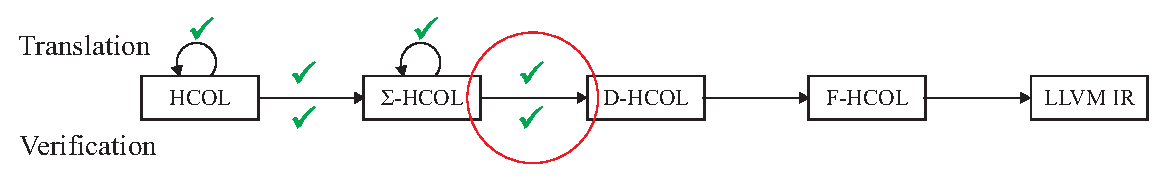
\includegraphics[keepaspectratio=true,width=0.96\paperwidth]{figures/lang_seq_to_dhcol.eps}
  \end{figure}

  {\SHCOL} language is shallow embedded, while {\DHCOL} is deep
  embedded. We were looking for a translation technique between the
  two which is:
  \medskip
  \begin{enumerate}
  \item Automated - Can automatically translate arbitrary valid
    {\SHCOL} expressions.
  \item Verified - Provides semantic preservation guarantees.
  \end{enumerate}

  \note[item]{{\SHCOL} and {\HCOL} are operator languages given
    denotational semantics and shallow embedding is convenient 
    representation for reasoning about them.}
  \note[item]{Translation validation is used for {\SHCOL} and
    {\HCOL} verification, while we develop a cerfified compiler from
    {\DHCOL} to LLVM IR}
  \note[item]{{\DHCOL} has only operational semantics}

\end{frame}

\begin{frame}[fragile]{An Example of Shallow Embedding in Coq}

  As an example let us consider a simple language of arithmetic
  expressions on natural numbers. It is shallow-embedded in Gallina
  and includes constants, bound variables, and three arithmetic
  operators: $+$, $-$, and $*$.
  
  \medskip
  Provided that $a, b, c, x \in \N$, the expression below is an
  example of a valid expression in the source language:
  \medskip
  \begin{lstlisting}[language=Coq, mathescape=true, basicstyle=\large,
    frame=single]
    2 + a*x*x + b*x + c.
  \end{lstlisting}

\end{frame}

\begin{frame}[fragile]{An Example of Deep Embedding in Coq}

  A deep-embedded variant of the same language includes the same
  operators but will be defined by an inductive type of its AST:

  \begin{lstlisting}[language=Coq, mathescape=true,
    frame=single, basicstyle=\footnotesize]
    Inductive NExpr: Type :=
    | NVar  : nat -> NExpr 
    | NConst: nat -> NExpr
    | NPlus : NExpr -> NExpr -> NExpr
    | NMinus: NExpr -> NExpr -> NExpr
    | NMult : NExpr -> NExpr -> NExpr.
  \end{lstlisting}

  Our sample expression, in deep-embedded target language, looks like:
  
  \begin{lstlisting}[language=Coq, mathescape=true,
    basicstyle=\footnotesize, frame=single]
    NPlus (NPlus (NPlus (NConst 2)
      (NMult (NMult (NVar 3) (NVar 0)) (NVar 0)))
        (NMult (NVar 2) (NVar 0))) (NVar 1)
  \end{lstlisting}
  
\end{frame}

\begin{frame}{Template Coq}
  TBD
\end{frame}

\begin{frame}[fragile]{Reification Approach}
  
  \begin{itemize}
  \item Implemented as \textit{Template Program} named \emph{reifyNExp}
  \item The input expressions are given in a closed form, where all
    variables first need to be introduced via lambda
    bindings. E.g. $\mathbb{N}$ or
    $\N \rightarrow \ldots \rightarrow \N$.
  \item \emph{reifyNExp} also takes two names (as strings). The first
    is used as the name of a new definition, to which the expression
    in the target language will be bound. The second is the name to
    which the semantic preservation lemma will be bound.
  \end{itemize}

  \begin{lstlisting}[language=Coq, mathescape=true, frame=single]
  Polymorphic Definition reifyNExp@{t u}
    {A:Type@{t}} (res_name lemma_name: string) (nexpr:A)
    : TemplateMonad@{t u} unit.
  \end{lstlisting}

  When executed, if successful, \emph{reifyNExp} will create a new
  definition and new lemma with the given names. If not, it will fail
  with an error. \note{The reason for a failure might be that the
    expression contains constructs which are legal in Gallina but not
    part of our embedded language.}

\end{frame}


\begin{frame}[fragile]{Reification Implementation}
  
  \begin{itemize}
  \item All variables are converted into parameters via \emph{forall}.
  \item Gallina AST (as \textit{quoted} by TemplateCoq) of the
    original expression is traversed and an expression in target
    language is generated.
  \item Variable names are converted to de Bruijn indices.
  \end{itemize}
  \medskip
  Our sample expression will be compiled to the following
  deep-embedded form:
  
    \begin{lstlisting}[language=Coq, mathescape=true,frame=single]
    NPlus (NPlus (NPlus (NConst 2)
        (NMult (NMult (NVar 3) (NVar 0)) (NVar 0)))
        (NMult (NVar 2) (NVar 0))) (NVar 1)
  \end{lstlisting}

\end{frame}

\begin{frame}[fragile]{Semantic Preservation Approach}
  
  Semantics of our deep embedded language is defined by evaluation
  function:

  \begin{lstlisting}[language=Coq, mathescape=true,frame=single]
    Definition evalContext:Type := list nat.
    Fixpoint evalNexp ($\Gamma$:evalContext) (e:NExpr): option nat.
  \end{lstlisting}

  The semantic preservation is expressed as a heterogeneous relation
  between expressions in the source and target languages:

  \begin{lstlisting}[language=Coq, mathescape=true,frame=single]
    Definition NExpr_term_equiv ($\Gamma$: evalContext)
    (d: NExpr) (s: nat) : Prop := evalNexp $\Gamma$ d = Some s.
  \end{lstlisting}

  For our sample expression the following lemma will be generated:
  
  \begin{lstlisting}[language=Coq, mathescape=true,frame=single]
forall x c b a : nat, NExpr_term_equiv [x; c; b; a]
    NPlus (NPlus (NPlus (NConst 2)
        (NMult (NMult (NVar 3) (NVar 0)) (NVar 0)))
        (NMult (NVar 2) (NVar 0))) (NVar 1)
    (2 + a * x * x + b * x + c)
  \end{lstlisting}
  
  \note[item]{The evaluation may fail, for example, if the expression references a
    variable not present in the evaluation context.}
  \note[item]{All variables are converted into parameters via \emph{forall}}
\end{frame}

\begin{frame}[fragile]{Automated Proof of Semantic Preservation Lemma}

  The general idea is to define and prove semantic
  equivalence lemmas for each pair of operators. For example:

  \begin{lstlisting}[language=Coq, mathescape=true,frame=single, basicstyle=\footnotesize]
Lemma NExpr_mul_equiv ($\Gamma$: evalContext) {a b a' b' }:
  NExpr_term_equiv $\Gamma$ a a' -> NExpr_term_equiv $\Gamma$ b b' ->
  NExpr_term_equiv $\Gamma$ (NMult a b) (Nat.mul a' b').
\end{lstlisting}

Because the expressions in the original and target languages have the
same structure, such proof can be automated, for example by use of
\emph{eauto} tactic.
  
  \begin{figure}[h]
    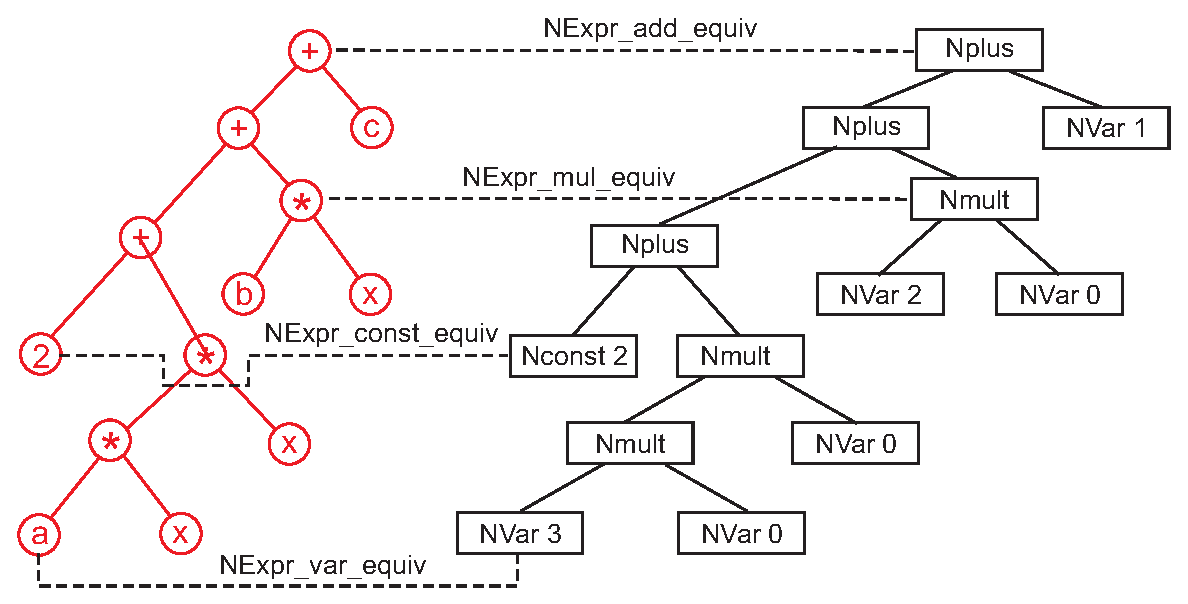
\includegraphics[width=0.5\columnwidth]{figures/trees.eps}
  \end{figure}

  \note{Compositional proof}
\end{frame}

\begin{frame}[fragile]{Questions?}

  Links:
  
  \begin{itemize}
  \item Full example: \url{https://github.com/vzaliva/CoqPL19-paper}
  \item TemplateCoq:
    \url{https://github.com/Template-Coq/template-coq/}
  \item \textit{``HELIX: a case
    study of a formal verification of high performance program
    generation.''}, Vadim Zaliva, Franz Franchetti. FHPC 2018. 
  \end{itemize}

  Contact:

  \begin{itemize}
  \item Vadim Zaliva: \url{http://www.crocodile.org/lord/}
  \item Matthieu Sozeau: \url{https://www.irif.fr/~sozeau/}
  \end{itemize}  
  
\end{frame}

\section{Backup slides}

\begin{frame}{From Denotational to Operational Semantics}
  \begin{center}
    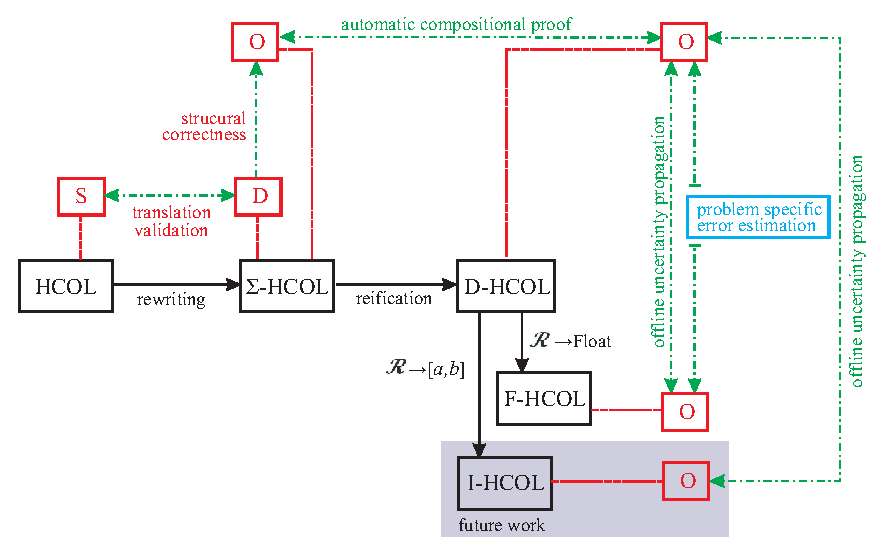
\includegraphics[width=0.8\columnwidth]{figures/semantics.eps}
  \end{center}
  
  \begin{enumerate}
  \item {\SHCOL} has both denotational and operational semantics.
  \item Structural properties allow to switch from one to another.
  \end{enumerate}
  
\end{frame}


\end{document}
